% ===================== AgentRx =====================
\subsection{AgentRx}\label{ds:agentrx}
\badgerow{\naturalbadge\ \partialbadge\ \lbl{agent + step + category}\ \lbl{single- and multi-agent}\ \lbl{$\tau$-bench retail / Magentic-One (Who\&When)}}

\begin{identity}
Paper & \emph{AgentRx: Diagnosing AI Agent Failures from Execution Trajectories} --- Barke, Goyal, Khare, Singh, Nath, Bansal (Microsoft Research / UIUC), EMNLP 2026 Findings, arXiv:2602.02475 \cite{agentrx2026}\\
Links & \href{https://huggingface.co/datasets/microsoft/AgentRx}{HF \code{microsoft/AgentRx}} (gated) \textperiodcentered\ \href{https://github.com/microsoft/AgentRx}{GitHub \code{microsoft/AgentRx}} \textperiodcentered\ \href{https://microsoft.com/en-us/research/blog/systematic-debugging-for-ai-agents-introducing-the-agentrx-framework}{MSR blog}\\
License & HF card CC BY 4.0; GitHub repository MIT\\
Status & HF download denied (approval required); the GitHub repo ships 73 of the paper's 170 annotated trajectories (29 $\tau$-bench retail + 44 Magentic-One) with identical schema---downloaded, 14 MB, \code{data/agentrx/github/data/}. Flash (42, internal Microsoft traces) and RelWork (45) are not released\\
\end{identity}

\paragraph{Description} AgentRx redefines the target as the \emph{critical failure step}---the first failure by any agent from which the run never recovers---and adds a \textbf{root-cause category}. The dataset is the evaluation set of the AgentRx debugging framework (constraint synthesis $\to$ step-wise checking $\to$ LLM judge). All failures are natural, from four domains:
\begin{itemize}
\item \textbf{$\tau$-bench retail} (39, 29 public): single tool-calling agent (gpt-4o) + simulated user under a domain policy; median 36 steps.
\item \textbf{Magentic-One} (44, all public): failed runs \emph{sampled from Who\&When's Hand-Crafted subset}; median 33 steps.
\item \textbf{Flash} (42) and \textbf{RelWork} (45; five trajectories from each of nine MAST / Who\&When settings): not public.
\end{itemize}
\textbf{Annotation}: grounded-theory open coding by three annotators in two phases---(1) exhaustive marking of \emph{every} step where an agent fails to make progress, including later-recovered ones; (2) identification of the critical failure and its category. Codes were merged until saturation, then frozen. On 30 trajectories labelled by all three, pairwise Cohen's $\kappa$ = 0.87--0.93 (\textbf{mean 0.89}); 20--24 min per trajectory. \textbf{Taxonomy} (9 categories, one per critical step, disambiguated by a yes/no checklist): Instruction/Plan Adherence, Invention of New Information, Invalid Invocation, Misinterpretation of Tool Output, Intent--Plan Misalignment, Under-specified User Intent, Intent Not Supported, Guardrails Triggered, System Failure. Labels: per-failure \code{step\_number}, \code{failed\_agent}, \code{failure\_category} and reasons; one \code{root\_cause} per trajectory.

\paragraph{Metrics and baselines} Exact step accuracy, Acc@$\pm$1/3/5, average step distance; category accuracy against the critical failure (also against any / earliest / terminal failure); failed-agent accuracy. gpt-5 judge, mean of 3 runs, in \% (paper). W\&W$^*$ = the Who\&When all-at-once prompt adapted to the first-unrecoverable definition.

\begin{center}\small
\begin{tabular}{@{}llccc@{}}\toprule
Domain & Method & Agent & Step & Cat.\\\midrule
$\tau$-bench & W\&W$^*$ & 65.0 & 18.8 & --\\
 & AgentRx & 66.7 & \textbf{42.7} & 47.0\\
Magentic & W\&W$^*$ & 61.4 & 22.7 & --\\
 & AgentRx & 71.2 & \textbf{36.4} & 46.2\\
Flash & AgentRx & 82.5 & 82.5 & 65.9\\
RelWork & AgentRx & 65.9 & 61.5 & 59.3\\\bottomrule
\end{tabular}
\end{center}
A judge-only ablation (no constraint evidence) drops step accuracy to 29.9 ($\tau$) and 32.6 (Magentic).

\paragraph{Schema} GitHub \code{data/}: \code{ground\_truth/tau\_ground\_truth.json} (29) and \code{magentic\_one\_ground\_truth.json} (44), each a list of \{\code{trajectory\_id}, \code{failure\_summary}, \code{failures}: [\{\code{failure\_id}, \code{step\_number}, \code{step\_reason}, \code{failure\_category}, \code{category\_reason}, \code{failed\_agent}\}], \code{root\_cause}: \{\code{failure\_id}, \code{reason\_for\_root\_cause}\}\}. Trajectories: \code{tau\_retail/tau\_dataset\_failed.json} (OpenAI chat messages with \code{tool\_calls}; \code{step\_number} is 1-based and counts the system message) and \code{magentic\_dataset/<id>.json} (lists of \{\code{content}, \code{role}\} with roles such as \code{Orchestrator (thought)}, \code{Orchestrator (-> WebSurfer)}, \code{WebSurfer}). Domain policies and tool schemas are included. The gated HF files (\code{tau\_retail.jsonl}, \code{magentic\_one.jsonl}) use the same fields plus \code{num\_failures}.

\paragraph{Statistics} computed from the public GitHub subset (73 trajectories); Flash and RelWork numbers are paper-only.\par\nobreak\vspace{1pt}
\noindent\begin{minipage}[t]{0.48\linewidth}\vspace{0pt}\small
\begin{tabular}{@{}lrrr@{}}\toprule
 & All & $\tau$-retail & Magentic\\\midrule
trajectories (all failed) & 73 & 29 & 44\\
steps: mean / median & 44.7 / 33 & 36.7 / 36 & 50.0 / 31.5\\
steps: min -- max & 5 -- 130 & 20 -- 62 & 5 -- 130\\
distinct agents: mean (max) & 3.3 (5) & 3 (3) & 3.4 (5)\\
failure events / traj.: mean (max) & 4.6 (55) & 1.3 (4) & 6.7 (55)\\
root step (1-based): mean / median & 18.5 / 17 & 24.7 / 21 & 14.4 / 10.5\\
relative root position: mean & 0.55 & 0.67 & 0.47\\
root = first annotated failure & 73\% & 93\% & 59\%\\
characters / traj.: mean & 46\,k & 18.7\,k & 64\,k\\\bottomrule
\end{tabular}

\smallskip Blamed agent: $\tau$-retail Assistant 21, \emph{User} 8 (under-specified intent); Magentic-One Orchestrator 23, WebSurfer 18, Assistant 2, FileSurfer 1. Over all 335 annotated failure events, Adherence failures dominate (203), but at the root cause Misinterpretation of Tool Output leads (22 of 73). Paper-reported sizes: 4.9\,k ($\tau$), 6.4\,k (Flash), 16.5\,k (Magentic) tokens per trajectory.
\end{minipage}\hfill
\begin{minipage}[t]{0.50\linewidth}\vspace{0pt}
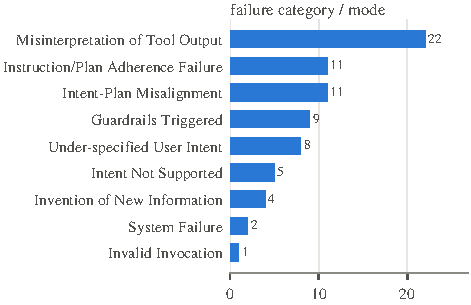
\includegraphics[width=\linewidth]{3_core/agentrx/figures/cat.pdf}
\end{minipage}

\paragraph{Example trajectory} Magentic-One log \code{e6bc9808\ldots} (8 steps, 3 roles, 9.2\,k characters) with two annotated failures: the WebSurfer reads only 35\% of the search page (step 5, Adherence), then the Orchestrator declares the request satisfied on that partial evidence (step 7, Misinterpretation)---the second event is the root cause, illustrating the first-\emph{unrecoverable}-failure convention. The run answers \$1.08 billion.
% auto-generated by scripts/render_traj.py -- do not edit
\trajtask{magentic\_one/\allowbreak{}e6bc98089608217e45b6956a46518fe3cce64a799b3ac43c6974c449ae14c408}{What's the highest price a high-rise apartment was sold for in Mission Bay,\allowbreak{} San Francisco,\allowbreak{} in 2021?\allowbreak{}}
\begin{trajstep}{1}{human}{agA}
What's the highest price a high-rise apartment was sold for in Mission Bay,\allowbreak{} San Francisco,\allowbreak{} in 2021?\allowbreak{}
\end{trajstep}
\begin{trajstep}{2}{Orchestrator (thought)}{agB}
Initial plan:\allowbreak{}\par We are working to address the following user request:\allowbreak{}\par What's the highest price a high-rise apartment was sold for in Mission Bay,\allowbreak{} San Francisco,\allowbreak{} in 2021?\allowbreak{}\par To answer this request we have assembled the following team:\allowbreak{}\par Assistant:\allowbreak{} A helpful and general-purpose AI assistant that has strong language skills,\allowbreak{} Python skills,\allowbreak{} and Linux command line skills.\newline ComputerTerminal:\allowbreak{} A computer terminal that performs no other action than running Python scripts (provided to it quoted in ```python code blocks),\allowbreak{} or sh shell scripts (provided to it quoted in ```sh code blocks)\newline FileSurfer:\allowbreak{} An agent that can handle local files.\newline WebSurfer:\allowbreak{} A helpful\newline [...] (1,\allowbreak{}675 chars omitted) [...]\newline /\allowbreak{}usr/\allowbreak{}local/\allowbreak{}lib/\allowbreak{}python3.11/\allowbreak{}site-packages/\allowbreak{}autogen\_magentic\_one/\allowbreak{}agents/\allowbreak{}orchestrator.py:\allowbreak{}216:\allowbreak{} UserWarning:\allowbreak{} Resolved model mismatch:\allowbreak{} gpt-4o-2024-08-06 !=\allowbreak{} gpt-4o-2024-05-13. Model mapping may be incorrect.\newline ledger\_response =\allowbreak{} await self.\_model\_client.create(
\end{trajstep}
\begin{trajstep}{3}{Orchestrator (thought)}{agB}
Updated Ledger:\allowbreak{}\newline \{\newline "is\_request\_satisfied":\allowbreak{} \{\newline "reason":\allowbreak{} "The request has not been satisfied as we have not yet identified the highest selling price for a high-rise apartment in Mission Bay,\allowbreak{} San Francisco,\allowbreak{} in 2021.",\allowbreak{}\newline "answer":\allowbreak{} false\newline \},\allowbreak{}\newline "is\_in\_loop":\allowbreak{} \{\newline "reason":\allowbreak{} "The tasks and questions are progressing towards finding the information,\allowbreak{} and there's no indication of repeating actions yet.",\allowbreak{}\newline "answer":\allowbreak{} false\newline \},\allowbreak{}\newline "is\_progress\_being\_made":\allowbreak{} \{\newline "reason":\allowbreak{} "We are making progress by planning to use WebSurfer to search for the specific information via relevant real estate databases and news sources.",\allowbreak{}\newline "answer":\allowbreak{} true\newline \},\allowbreak{}\newline "\newline [...] (391 chars omitted) [...]\newline the highest price a high-rise apartment was sold for in Mission Bay,\allowbreak{} San Francisco,\allowbreak{} in 2021. Check websites like Zillow,\allowbreak{} Redfin,\allowbreak{} Realtor.com,\allowbreak{} or local news outlets like the San Francisco Chronicle. Report back the highest selling price you find."\newline \}\newline \}
\end{trajstep}
\begin{trajstep}{4}{Orchestrator (-> WebSurfer)}{agC}
Please search for the highest price a high-rise apartment was sold for in Mission Bay,\allowbreak{} San Francisco,\allowbreak{} in 2021. Check websites like Zillow,\allowbreak{} Redfin,\allowbreak{} Realtor.com,\allowbreak{} or local news outlets like the San Francisco Chronicle. Report back the highest selling price you find.
\end{trajstep}
\begin{trajstep}{5}{WebSurfer}{agD}
I typed 'highest price high-rise apartment sold Mission Bay San Francisco 2021' into '0 characters out of 2000'.\par Here is a screenshot of [highest price high-rise apartment sold Mission Bay San Francisco 2021 - Search](https:\allowbreak{}/\allowbreak{}/\allowbreak{}www.bing.com/\allowbreak{}search?\allowbreak{}q=\allowbreak{}highest+price+high-rise+apartment+sold+Mission+Bay+San+Francisco+2021\&form=\allowbreak{}QBLH\&sp=\allowbreak{}-1\&lq=\allowbreak{}0\&pq=\allowbreak{}\&sc=\allowbreak{}0-0\&qs=\allowbreak{}n\&sk=\allowbreak{}\&cvid=\allowbreak{}A0A2F14E955F4D08B290B29A975075DF\&ghsh=\allowbreak{}0\&ghacc=\allowbreak{}0\&ghpl=\allowbreak{}). The viewport shows 35\% of the webpage,\allowbreak{} and is positioned at the top of the page.\newline The following metadata was extracted from the webpage:\allowbreak{}\par \{\newline "meta\_tags":\allowbreak{} \{\newline "referrer":\allowbreak{} "origin-when-cross-origin",\allowbreak{}\newline "SystemEntrop\newline [...] (2,\allowbreak{}924 chars omitted) [...]\newline icon)\newline +1 415-738-7000 (phone icon)\newline Suggest an edit button\newline Your business?\allowbreak{} Claim now (edit icon)\newline Add more information\newline Add website link\newline Add hours link\newline Add photos link\par People also search for:\allowbreak{}\par Images below\par Yelp logo\newline Yelp page for another business\newline <Image>
\end{trajstep}
\begin{trajstep}{6}{Orchestrator (thought)}{agB}
Updated Ledger:\allowbreak{}\newline \{\newline "is\_request\_satisfied":\allowbreak{} \{\newline "reason":\allowbreak{} "The highest price found for a high-rise apartment sold in Mission Bay,\allowbreak{} San Francisco,\allowbreak{} in 2021,\allowbreak{} is \$1.08 billion for 1800 Owens Street.",\allowbreak{}\newline "answer":\allowbreak{} true\newline \},\allowbreak{}\newline "is\_in\_loop":\allowbreak{} \{\newline "reason":\allowbreak{} "The request has been successfully addressed with the required information.",\allowbreak{}\newline "answer":\allowbreak{} false\newline \},\allowbreak{}\newline "is\_progress\_being\_made":\allowbreak{} \{\newline "reason":\allowbreak{} "The request has been resolved with the discovery of the highest selling price.",\allowbreak{}\newline "answer":\allowbreak{} true\newline \},\allowbreak{}\newline "next\_speaker":\allowbreak{} \{\newline "reason":\allowbreak{} "The request has been fulfilled.",\allowbreak{}\newline "answer":\allowbreak{} "Assistant"\newline \},\allowbreak{}\newline "instruction\_or\_question":\allowbreak{} \{\newline "reason":\allowbreak{} "The necessary information has been found.",\allowbreak{}\newline "answer":\allowbreak{} "The highest price a high-rise apartment was sold for in Mission Bay,\allowbreak{} San Francisco,\allowbreak{} in 2021,\allowbreak{} is \$1.08 billion for 1800 Owens Street."\newline \}\newline \}
\end{trajstep}
\begin{faultystep}{7}{Orchestrator (thought)}{agB}
Request satisfied.
\end{faultystep}
\begin{trajstep}{8}{Orchestrator (termination condition)}{agE}
No agent selected.\newline /\allowbreak{}workspace/\allowbreak{}scenario.py:\allowbreak{}94:\allowbreak{} UserWarning:\allowbreak{} Resolved model mismatch:\allowbreak{} gpt-4o-2024-08-06 !=\allowbreak{} gpt-4o-2024-05-13. Model mapping may be incorrect.\newline response =\allowbreak{} await client.create(messages)\newline FINAL ANSWER:\allowbreak{} 1080000000\newline SCENARIO.PY COMPLETE !\#!\#\newline RUN.SH COMPLETE !\#!\#
\end{trajstep}
\trajannotation{Orchestrator}{7}{Misinterpretation of Tool Output}{Orchestrator said request satisfied on incomplete information | category\_reason:\allowbreak{} Orchestrator said request satisfied without on incomplete information even though websurfer had worked on partial webpage | root\_cause:\allowbreak{} The orchestrator failed to ensure that the websurfer had gathered complete information before concluding that the request was satisfied.}{—}{No agent selected.\newline /\allowbreak{}workspace/\allowbreak{}scenario.py:\allowbreak{}94:\allowbreak{} UserWarning:\allowbreak{} Resolved model mismatch:\allowbreak{} gpt-4o-2024-08-06 !=\allowbreak{} gpt-4o-2024-05-13. Model mapping may be incorrect.\newline response =\allowbreak{} await client.creat\newline [...] (10 chars omitted) [...]\newline )\newline FINAL ANSWER:\allowbreak{} 1080000000\newline SCENARIO.PY COMPLETE !\#!\#\newline RUN.SH COMPLETE !\#!\#}{\textbf{all\_failures}: [\{"failure\_id":\allowbreak{} 1,\allowbreak{} "step\_number":\allowbreak{} 5,\allowbreak{} "step\_reason":\allowbreak{} "Webusurfer worked on 35\% of the webpage",\allowbreak{} "failure\_category":\allowbreak{} "Instruction/\allowbreak{}Plan Adherence Failure",\allowbreak{} "category\_reason":\allowbreak{} "Websurfer worked on 35\% of the webpage despite orchestrator asking for complete information",\allowbreak{} "failed\_agent":\allowbreak{} "Websurfer"\},\allowbreak{} \{"failure\_id":\allowbreak{} 2,\allowbreak{} "step\_number":\allowbreak{} 7,\allowbreak{} "step\_reason":\allowbreak{} "Orchestrato\newline [...] (145 chars omitted) [...]\newline d request satisfied without on incomplete information even though websurfer had worked on partial webpage",\allowbreak{} "failed\_agent":\allowbreak{} "Orchestrator"\}]; \textbf{root\_cause}: \{"failure\_id":\allowbreak{} 2,\allowbreak{} "reason\_for\_root\_cause":\allowbreak{} "The orchestrator failed to ensure that the websurfer had gathered complete information before concluding that the request was satisfied."\}; \textbf{failure\_summary}: The orchestrator prematurely concluded that the user's request was satisfied based on incomplete data provided by the websurfer agent.; \textbf{step\_indexing}: step\_number is a 1-based index into the message list;\allowbreak{} tau-bench list includes the system (policy) message at step 1; \textbf{canonical\_category}: Misinterpretation of Tool Output}


\paragraph{Notes} (i) Only partially public: HF is gated and the released GitHub subset covers 73 of 170 trajectories; the proprietary Flash traces, where AgentRx scores highest, cannot be inspected. (ii) The root cause is not the first failure in 27\% of public trajectories (41\% of Magentic-One), because orchestrators recover from early mistakes; the paper's example 5f982798 is labelled step 3 by Who\&When and step 33 by AgentRx. (iii) All 44 Magentic-One logs come from Who\&When Hand-Crafted (16 are stored in Who\&When format), so results on the two benchmarks are not independent. (iv) Every failure event is annotated (up to 55 per trajectory), enabling earliest/any/terminal-failure metrics. (v) Label hygiene: category strings vary (\code{Instruction Adherence Failure} vs \code{Instruction/Plan Adherence Failure}, \code{Underspecified} vs \code{Under-specified}, \code{Websurfer} vs \code{WebSurfer}); one \code{failure\_id} is a string; \code{failed\_agent} may be the simulated \code{User}. (vi) Few agents per trajectory, so the informative targets are step and category; the same pipeline was also run on all 1,022 MAST trajectories without gold labels.
